\documentclass[aspectratio=1610,20pt,utf8]{beamer}
\setbeamersize{text margin left=5pt,text margin right=5pt}
\setbeamerfont{subsection in toc}{size=\small}
\usepackage[utf8]{inputenc}
\usepackage[T1]{fontenc}
\usepackage[USenglish]{babel}
\usepackage{graphicx} % graphics
\usepackage{array, tabularx, caption, boldline}
\usepackage{mathabx}
\usepackage{mathpazo}
\usepackage{eulervm}
\usepackage{tikz} %for the points
\usepackage{amssymb}

\newcommand{\shrug}[1][]{%
	\begin{tikzpicture}[baseline,x=0.8\ht\strutbox,y=0.8\ht\strutbox,line width=0.125ex,#1]
	\def\arm{(-2.5,0.95) to (-2,0.95) (-1.9,1) to (-1.5,0) (-1.35,0) to (-0.8,0)};
	\draw \arm;
	\draw[xscale=-1] \arm;
	\def\headpart{(0.6,0) arc[start angle=-40, end angle=40,x radius=0.6,y radius=0.8]};
	\draw \headpart;
	\draw[xscale=-1] \headpart;
	\def\eye{(-0.075,0.15) .. controls (0.02,0) .. (0.075,-0.15)};
	\draw[shift={(-0.3,0.8)}] \eye;
	\draw[shift={(0,0.85)}] \eye;
	% draw mouth
	\draw (-0.1,0.2) to [out=15,in=-100] (0.4,0.95); 
	\end{tikzpicture}}
\newcommand*\circled[1]{\tikz[baseline=(char.base)]{\node[shape=circle,draw,inner sep=2pt] (char) {#1};}}

\usetheme{unipassau}


% title slide definition
\title[Team Hams]{Sprint 03}
\subtitle{Design}
\author[\today]{Andreas M\"uller}
\institute[Team Hams]
{
  Team Hams\\
  Leading Product Owner and Scrum Master\\
}
\date{23.11.2018}

%--------------------------------------------------------------------
%                            Titlepage
%--------------------------------------------------------------------

\begin{document}

\begin{frame}[plain]
  \titlepage
\end{frame}

\begin{frame}{Overview}
\tableofcontents
\end{frame}

%-------------------------------------------------------------------
%                            Content
%-------------------------------------------------------------------
%%%%%%%%%%%%%%%%%%%%%%%%%%%%%%%%%%%%%%%%%%%%%%%%%%%%%%%%%%%%%%%%%%%%%%
\section{Sprint} 
%--------------------------------------------------------------------%

\subsection{Burndown}
\begin{frame}{Burndown Jira}
	\centering
	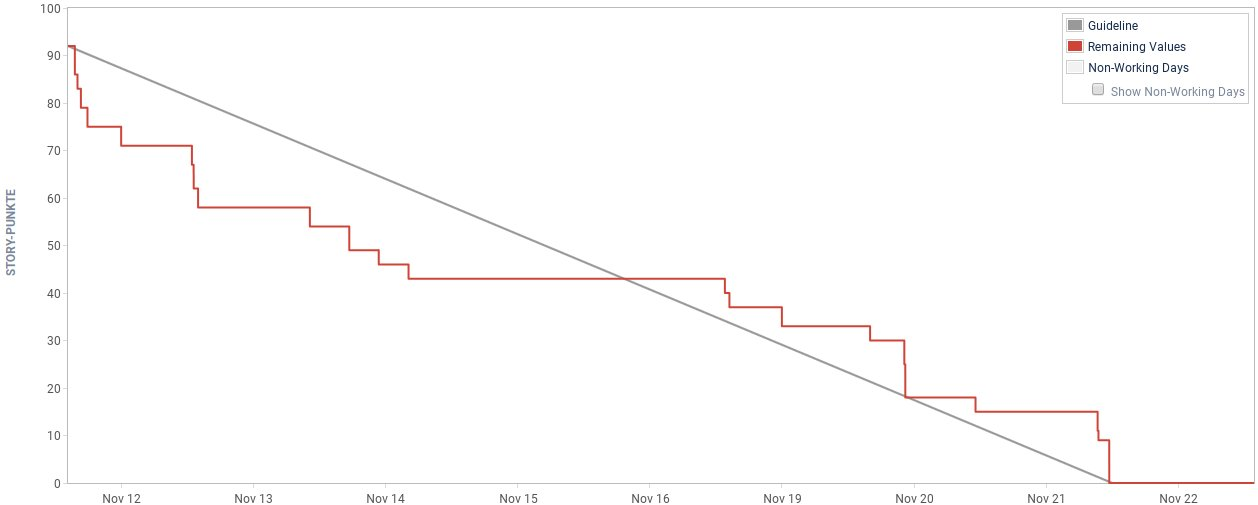
\includegraphics[width=15cm]{img/s03_hams_jira_burndown.jpg}
\end{frame}

\subsection{User Stories}
\begin{frame}
	\frametitle{User Stories}
	\begin{minipage}{15cm}
		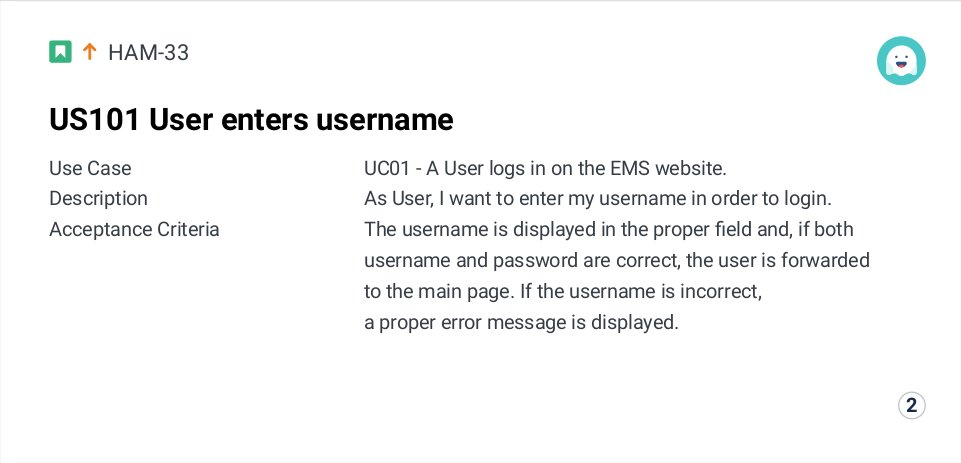
\includegraphics[width=15cm]{img/user_story_101.jpg}
		\centering
	\end{minipage}%
\end{frame}
%%%%%%%%%%%%%%%%%%%%%%%%%%%%%%%%%%%%%%%%%%%%%%%%%%%%%%%%%%%%%%%%%%%%%%
\section{Product}
%--------------------------------------------------------------------%
\subsection{User Types}
\begin{frame}
	\frametitle{User Types}
	\begin{minipage}{15cm}
		\includegraphics[width=13cm]{img/s03_hams_usergroups.pdf}
		\centering
	\end{minipage}%
\end{frame}

%%%%%%%%%%%%%%%%%%%%%%%%%%%%%%%%%%%%%%%%%%%%%%%%%%%%%%%%%%%%%%%%%%%%%%

\subsection{Domain Diagram}
\begin{frame}
	\frametitle{Domain Diagram}
	\includegraphics[width=15cm]{img/s03_hams_be-domainclasses.pdf}
	\centering
\end{frame}

%%%%%%%%%%%%%%%%%%%%%%%%%%%%%%%%%%%%%%%%%%%%%%%%%%%%%%%%%%%%%%%%%%%%%%

\subsection{JWT Authentication}
\begin{frame}
	\frametitle{JWT Authentication}
	\begin{itemize}
		\item Access-Token
		\begin{itemize}
			\item holds state
			\item short lived e.g. 1 hour
		\end{itemize}
		\item Refresh-Token
		\begin{itemize}
			\item used to gets new Access-Token
			\item long lived e.g. 1 day
		\end{itemize}
	\end{itemize}
\end{frame}

%%%%%%%%%%%%%%%%%%%%%%%%%%%%%%%%%%%%%%%%%%%%%%%%%%%%%%%%%%%%%%%%%%%%%%

\subsection{Last Feedback}
\begin{frame}
	\frametitle{Last Feedback}
	\begin{itemize}
		\item Resolution
		\begin{itemize}
			\item change size of time frame
			\item smoothing as Extended Criteria
		\end{itemize}
		\item Password reset
		\begin{itemize}
			\item was not in our Base Criteria
		\end{itemize}
	\end{itemize}
\end{frame}

%%%%%%%%%%%%%%%%%%%%%%%%%%%%%%%%%%%%%%%%%%%%%%%%%%%%%%%%%%%%%%%%%%%%%%
\section{Prototype}
%--------------------------------------------------------------------%

\end{document}
